\subsection{具体例: 実階数1の古典型単純Lie群の場合}
\begin{prop}\label{prop:classical-rank-one}
  $G = \SO(1,n)$,$ \SU(1, n)$,$\Sp(1,n) $,$H = \SO(1,1) $,$n\geq 2$に対して\Cref{prob:1121} は正しい.
\end{prop}

$G = \Sp(1,2) $,$\ha = \real \begin{pmatrix}
    0 & 1 & 0 \\
    1 & 0 & 0\\
    0 & 0 & 0
  \end{pmatrix}$の場合にのみ示す.その他の場合も全く同様の議論である.
\begin{prop}\label{prop:1127-main}
  $G = \Sp(1,2) $,$H = \SO(1,1)$,$X\in \pe$に対し,$Y(\real X) $が有界であることと$ X\in \{0\}\cup \pe\setminus \ha  $であることは同値である.
\end{prop}

ただし,$H$は$G$の左上に入っている.すなわち,$\ha = \real Y $,$Y\defeq \begin{pmatrix}
  0 & 1 & 0 \\
  1 & 0 & 0\\
  0 & 0 & 0
\end{pmatrix}$とする.

\begin{nttdef}\label{nttdef:1127-main}
  
  $\quat$を四元数体とする.${\Sp(1,2)\defeq \{g\in \GL(3,\quat)\mid \bar{\trans{g}}\; I_{1,2}g = I_{1,2}  \}} $,$I_{1,2} \defeq \diag(-1,1,1) $とし,$\Sp(1,2) $の$\quat^3 $への自然表現を,任意の$\begin{pmatrix}
    x_{11} & x_{12} & x_{13}\\ x_{21} & x_{22} & x_{23}\\ x_{31} & x_{32} & x_{33}
  \end{pmatrix}\in \Sp(1,2)$と任意の$\begin{pmatrix}
    a \\ b \\c
  \end{pmatrix}\in \quat^3 $に対し
  \begin{align*}
    \begin{pmatrix}
      x_{11} & x_{12} & x_{13}\\ x_{21} & x_{22} & x_{23}\\ x_{31} & x_{32} & x_{33}
    \end{pmatrix}\cdot
                                                                              \begin{pmatrix}
                                                                                a \\ b \\c
                                                                              \end{pmatrix}
    =
    \begin{pmatrix}
      x_{11}a + x_{12}b + x_{13}c\\ x_{21}a + x_{22}b + x_{23}c\\ x_{31}a + x_{32}b + x_{33}c\\    
    \end{pmatrix}
  \end{align*}
  により定める.
  
  $\Sp(1,2)/(\Sp(1)\times \Sp(2)) \simeq \{(z_1, z_2)\mid z_1,z_2\in \quat ,\; \abs{z_1}^2 + \abs{z_2}^2   < 1 \} =: \quat\mathbb{H}^2 $である.この$\Sp(1,2)/(\Sp(1)\times \Sp(2)) $と$\quat\mathbb{H}^2$の間の微分同相は$\trans{(1,0,0)} $の$\Sp(1,2)$軌道上の点$
  \begin{pmatrix}
    \zeta_0 \\ \zeta_1 \\ \zeta_2 
  \end{pmatrix}
  \in \quat^3$に対して$\quat\mathbb{H}^2$の点$\begin{pmatrix}
    \zeta_1\inv{\zeta_0} \\ \zeta_2 \inv{\zeta_0}
  \end{pmatrix}$を対応させることで得られる.

  $\trans{(1,0,0)} $の$\Sp(1,2)$軌道上の点$
  \begin{pmatrix}
    \zeta_0 \\ \zeta_1 \\ \zeta_2 
  \end{pmatrix}
  \in \quat^3 $に対応する$\quat\mathbb{H}^2$の点を$\lbig[
  \begin{pmatrix}
    1 \\ \zeta_1\inv{\zeta_0} \\ \zeta_2 \inv{\zeta_0}
  \end{pmatrix}\rbig]
  $とも書く.
  
  % により対応させることで得られる.
  % $\trans{(1,0,0)} $の自然表現$\Sp(1,2)\leftaction \quat^3 $による軌道を考え,第2,第3成分に第1成分の逆数を右からかけた空間が$\quat\mathbb{H}^2$と微分同相であるためである.対応すると書く.
\end{nttdef}

行列計算により,次が示される.
\begin{lem}\label{lem:exp-quat}
  
  任意の$ z,w\in \quat$に対し,
  \begin{align*}
    \exp
    \begin{pmatrix}
      0 & z & w  \\
      \bar{z} & 0 & 0\\
      \bar{w} & 0 & 0
    \end{pmatrix}
                    =
                    \begin{pmatrix}
                      \cosh r &  \dfrac{z}{r} \sinh r & \dfrac{w}{r}\sinh r \\
                      \\
                      \dfrac{\bar{z}}{r} \sinh r & \dfrac{\abs{w}^2 + \abs{z}^2\cosh r}{r^2}  & \dfrac{\bar{z}w(\cosh r -1)}{r^2} \\
                      \\
                      \dfrac{\bar{w}}{r}\sinh r &  \dfrac{\bar{w}z(\cosh r -1)}{r^2} & \dfrac{\abs{z}^2 + \abs{w}^2\cosh r}{r^2} 
                    \end{pmatrix}
  \end{align*}
  である.ただし$r \defeq \sqrt{\abs{z}^2 + \abs{w}^2 } $とする.
\end{lem}

\begin{npfwn}[\Cref{prop:1127-main}]
  
  % $\Lie H = \ha = \real A $,$A\defeq \begin{pmatrix}
  %   0 & 1 & 0 \\
  %   1 & 0 & 0\\
  %   0 & 0 & 0
  % \end{pmatrix}$とする.
  $X = 0$ならば$ Y(\real X) = \{0\} $である.また$X\in \ha\setminus\{0\} $のときに$Y(\real X) $が非有界であることは明らかであるから,$X\nin \ha $の場合にのみ議論すればよい.したがって$\abs{z_0}^2 +\abs{w_0}^2  = 1 $かつ$ z_0 \neq \pm 1 $を満たす$z_0,w_0\in \quat$により$X =  \begin{pmatrix}
    0 & z_0 & w_0 \\
    \bar{z_0} & 0 & 0 \\
    \bar{w_0} & 0 & 0 
  \end{pmatrix}$と書かれている$X$に対して$Y(\real X) $の有界性を議論して一般性を失わない ($\abs{z_0}^2 +\abs{w_0}^2  = 1 $を仮定したとき$X\nin \ha $であることと$z_0\neq \pm 1$であることは同値である).以下,$X$はこのように書ける元とする.% つまり
  % $X =
  % \begin{pmatrix}
  %   0 & z & w \\
  %   \bar{z} & 0 & 0 \\
  %   \bar{w} & 0 & 0 
  % \end{pmatrix}
  % \in \pe\setminus\ha $,$z,w\in \quat \st \abs{z}^2 +\abs{w}^2  = 1 $を任意に1つ固定して議論して一般性を失わない.このとき,$X\in\pe\setminus \ha $より$\re z \neq \pm 1$であることに注意する ($\re\colon \quat\ni a+bi+cj+dk\mapsto a\in \real$とする).

  $G$の Cartan 対合を$\Theta(g) = \inv{(g^{*})} $ ($g^{*}$は$g$の共役転置) とするとき,$\Theta(e^{Y(tX)}e^{Z(tX)})\cdot o_K = e^{-Y(tX)}e^{-Z(tX)}\cdot o_K = \Theta(e^{tX})\cdot o_K = e^{-tX}\cdot o_K $より,$Y(\real X) $が非有界であることと$ Y(\real X)\subset \real Y $が上に非有界であることは同値である.

  したがって,$Y (\real X) $が非有界であるとき,必要なら部分列を取り,$Y$の符号を入れ替えて,列$\{t_n \in \real_{\geq 0} \}_{n\in \nat} $で,$t_n\to \infty$かつ$s_n\to \infty$,$ n\to \infty$,ただし$Y(t_n X) = s_n Y$,なるものが存在する.

  任意の$\per{\ha}\cap\pe $の元はある$Z =
  \begin{pmatrix}
    0 & z & w \\
    \bar{z} & 0 & 0 \\
    \bar{w} & 0 & 0 
  \end{pmatrix} \in \per{\ha}\cap\pe $ (ただし$z,w\in \quat$は$ \abs{z}^2 +\abs{w}^2  = 1 $を満たす) と$r\in \real$により$rZ$と表せる.よって$Z(t_nX) = r_nZ_n$,$Z_n\defeq \begin{pmatrix}
    0 & z_n & w_n \\
    \bar{z_n} & 0 & 0 \\
    \bar{w_n} & 0 & 0 
  \end{pmatrix} $ (ただし$z_n,w_n\in \quat $は$ \abs{z_n}^2 +\abs{w_n}^2  = 1 $を満たし,$r_n\in \real$とする) の形で表わせる.$X\nin\ha$であるから\Cref{thm:kob97}より$\abs{r_n}\to \infty $,$n\to \infty$である.$z_n,w_n\in \quat $は$ \abs{z_n}^2 +\abs{w_n}^2  = 1 $を満たすから,$\{t_n\} $の部分列を取るとある$z_{\infty},w_{\infty}\in\quad $が存在して$Z_{\infty}\defeq \lim_{n\to \infty}Z_n  =
  \begin{pmatrix}
    0 & z_{\infty} & w_{\infty} \\
    \bar{z_{\infty}} & 0 & 0 \\
    \bar{w_{\infty}} & 0 & 0 
  \end{pmatrix}
  \in \per{\ha}\cap\pe $,$\abs{z_{\infty}}^2 +\abs{w_{\infty} }^2  = 1$なるようにできる.$Z_{\infty}\in \per{\ha}\cap\pe$,特に$Z_{\infty} \in\pe\setminus \ha $より$\re z_{\infty} \neq \pm 1$であることに注意する ($\re\colon \quat\ni a+bi+cj+dk\mapsto a\in \real$とする).

  \Cref{lem:exp-quat}より, 
  \begin{align*}
    e^{s_n Y}e^{r_n Z_n}\cdot o_K &=
    \begin{pmatrix}
      \cosh s_n & \sinh s_n & 0 \\
      \sinh s_n & \cosh s_n & 0 \\
      0 & 0 & 1 
    \end{pmatrix}
              \lbig[\begin{pmatrix}
                1\\ \pm \bar{z_n} \tanh \abs{r_n}  \\ \pm \bar{w_n} \tanh \abs{r_n}
              \end{pmatrix}\rbig]\\
    &=  \lbig[ \begin{pmatrix}
      \cosh s_n \pm \bar{z_n} \tanh \abs{r_n} \sinh s_n \\ \sinh s_n \pm \bar{z_n} \tanh \abs{r_n} \cosh s_n \\ \pm \bar{w_n} \tanh \abs{r_n}
    \end{pmatrix}\rbig]
  \end{align*}
  である.ただし複号は$r_n$の符号$\pm$と同順である.このとき$\lim_{n\to \infty}\tanh s_n = 1 = \lim_{n\to \infty}\tanh \abs{r_n} $と$\lim_{n\to \infty} \re z_n = \re z_{\infty} \neq \pm 1$に注意すると次を得る.
  \begin{align}
    \lim_{n\to \infty}(\sinh s_n \pm \bar{z_n} \tanh \abs{r_n} \cosh s_n)\inv{(\cosh s_n \pm \bar{z_n} \tanh \abs{r_n} \sinh s_n) } = 1.\label{eq:-1}
  \end{align}
  \Cref{eq:-1}を得るための具体的な計算は後述する.

  \Cref{eq:-1}より$
  \begin{pmatrix}
    0 \\ 0 
  \end{pmatrix}
  \in \quat\mathbb{H}^2 $から$
  \begin{pmatrix}
    1 \\ 0 
  \end{pmatrix}
  \in \quat\mathbb{H}^2 $へのベクトルと,$
  \begin{pmatrix}
    0 \\ 0 
  \end{pmatrix}
  \in \quat\mathbb{H}^2 $から\\
  $ \begin{pmatrix}
    (\sinh s_n \pm \bar{z_n} \tanh \abs{r_n} \cosh s_n)\inv{(\cosh s_n \pm \bar{z_n} \tanh \abs{r_n} \sinh s_n) } \\  \ast 
  \end{pmatrix}\in \quat\mathbb{H}^2 $へのベクトルがなすEuclid内積の値を $I_n$とすると,$\lim_{n\to \infty}I_n = 1 $である.

  $
  \begin{pmatrix}
    0 \\ 0 
  \end{pmatrix}
  \in \quat\mathbb{H}^2 $から$
  \begin{pmatrix}
    1 \\ 0
  \end{pmatrix}
  \in \quat\mathbb{H}^2 $へのベクトルと,$
  \begin{pmatrix}
    0 \\ 0 
  \end{pmatrix}
  \in \quat\mathbb{H}^2 $から$e^{t_nX}\cdot o_K \in \quat \mathbb{H}^2 $へのベクトルがなすEuclid内積の値$J_n$を計算する.$X =   \begin{pmatrix}
    0 & z_0 & w_0 \\
    \bar{z_0} & 0 & 0 \\
    \bar{w_0} & 0 & 0 
  \end{pmatrix}$ (ただし$\abs{z_0}^2 + \abs{w_0}^2 = 1 $かつ$z_0\neq \pm 1 $) と設定したことを思い出すと,\Cref{lem:exp-quat}より$J_n = \bar{z_0}\tanh t_n $である.$X\nin \ha $であることと$z_0\neq \pm 1$であることは同値であることと$t_n\to \infty$,$n\to \infty$より$\lim_{n\to \infty}J_n = \bar{z_0}\neq 1 $である.% ,$r_0\defeq \sqrt{\abs{z_0}^2 + \abs{w_0}^2 } $

  $e^{s_n Y}e^{r_n Z_n}\cdot o_K = e^{t_n X}\cdot o_K$より$ \lim_{n\to \infty} I_n = \lim_{n\to \infty}J_n  $であるが,以上2つの議論を合わせると$\lim_{n\to \infty} I_n= 1$,$\lim_{n\to \infty}J_n \neq 1 $となり矛盾する.
  

  以上より$X\in \pe\setminus\ha$ならば$Y(\real X) $は有界であり,\Cref{prop:1127-main} を得る.  
\end{npfwn}


\begin{ncalcof}[\Cref{prop:1127-main},\Cref{eq:-1}]
    
  \begin{align*}
    \lim_{n\to \infty}\abs{(\sinh s_n \pm \bar{z_n} \tanh \abs{r_n} \cosh s_n)\inv{(\cosh s_n \pm \bar{z_n} \tanh \abs{r_n} \sinh s_n) } - 1} = 0
  \end{align*}
  を示せば主張が得られる.具体的に計算すると,
  \begin{align}
    &\lim_{n\to \infty}\abs{(\sinh s_n \pm \bar{z_n} \tanh \abs{r_n} \cosh s_n)\inv{(\cosh s_n \pm \bar{z_n} \tanh \abs{r_n} \sinh s_n) } - 1}\notag \\
    % &\qquad\qquad\qquad \text{($\text{(この極限)} = 0$を示せば良い)} \\
    = & \lim_{n\to \infty}\lbig|\frac{(\tanh s_n\pm \bar{z_n}\tanh \abs{r_n})(1 \pm z_n \tanh\abs{r_n}\tanh s_n )}{\abs{(1 \pm \bar{z_n} \tanh\abs{r_n}\tanh s_n )}^2} - 1 \rbig|\label{eq:ast} \tag{$\ast$}  
  \end{align}
  である.ここで$ z_n'\defeq 1 \pm z_n\tanh\abs{r_n}\tanh s_n$とおくと,
  \begin{align*}
    (\ast)&=  \lim_{n\to \infty}\frac{\abs{(\tanh s_n\pm \bar{z_n}\tanh \abs{r_n})z_n' - (1 \pm \bar{z_n} \tanh\abs{r_n}\tanh s_n )z_n' }}{\abs{\bar{z_n'}}^2}\\
            % &= \lim_{n\to \infty}\frac{\abs{(\tanh s_n\pm \bar{z_n}\tanh \abs{r_n})z_n' - (1 \pm \bar{z_n} \tanh\abs{r_n}\tanh s_n )z_n' }}{\abs{\abs{\bar{z_n'}}}}\\
    &= \lim_{n\to \infty}\frac{\abs{(1-\tanh s_n)(-1\pm \bar{z_n}\tanh \abs{r_n} )z_n'}}{\abs{\bar{z_n'}}^2} \\
    &= \lim_{n\to \infty}\frac{\abs{(1-\tanh s_n)(-1\pm \bar{z_n}\tanh \abs{r_n} )}}{\abs{(1 \pm \bar{z_n} \tanh\abs{r_n}\tanh s_n )}} 
  \end{align*}
  である.
  $\lim_{n\to \infty} \re z_n = \re z_{\infty} \neq \pm 1$より,$0 < \min{\abs{1\pm \re z_n}}\leq  \abs{(1 \pm \bar{z_n} \tanh\abs{r_n}\tanh s_n )}\leq \sqrt{2^2 + 1^2} = \sqrt{5} $と$0< \min\{\abs{-1\pm \re z_n } \}  \leq \abs{-1\pm\bar{z_n}\tanh \abs{r_n} } \leq \sqrt{5} $であることより,
    \begin{align*}
      0 &= \lim_{n\to \infty}(1-\tanh s_n)\frac{\min\{\abs{-1\pm \re z_n} \}}{\sqrt{5}} \\
        &\leq \lim_{n\to \infty}\frac{\abs{(1-\tanh s_n)(-1\pm \bar{z_n}\tanh \abs{r_n} )}}{\abs{(1 \pm \bar{z_n} \tanh\abs{r_n}\tanh s_n )}}\\
      &\leq \lim_{n\to \infty}(1-\tanh s_n)\frac{\sqrt{5}}{\min\{\abs{1\pm \re z_n} \}} = 0
    \end{align*}
    を得,\Cref{eq:-1} が成り立つ.
\end{ncalcof}

\begin{cor}\label{cor:prob-eg}
  $G = \SO(1,n) $,$H = \SO(1,l) $,$1\leq l\leq n-1$は\Cref{prob:1121}の肯定的な例である.具体的には$\pe_{H,\bdd} = \{0\}\cup \pe\setminus\ha $である.ただし$H$は$G$の左上にブロック行列として実現する.
  % より具体的には次の\Cref{thm:1018-main}が成り立つ.
\end{cor}
% \begin{prop}\label{thm:1018-main}
%   % $\SO(n,1)/\SO(n) $を {\Poincare} ball model で実現したとき,
%   $G = \SO(1,n) $,$H = \SO(1,k) $,$1\leq k\leq n-1$,とする.
%   \begin{align*}
%     Y(X) =
%     \begin{cases}
%       \ds  \frac{1}{4}\inv{\tanh}[\tanh(4\norm{X})\cos\theta ]\frac{X_1}{\norm{X_1}}, &X\in \pe\setminus \per{\ha} \\
%     \ds  0, &X\in  \per{\ha}\cap \pe
%   \end{cases}
%   \end{align*}
%   である.
% \end{prop}
% \begin{cor}
%   % $X\in \pe\setminus \ha $
%   % % $ e^{X}\cdot o_K\nin \SO(k,1)\cdot o_K $
%   % に対し$0 \leq \cos \theta\neq 1$であり,
%   $X\in \pe\setminus\per{\ha}$ならば$0 < \cos \theta \leq 1$であり,
%   \begin{align*}
%     Y(\real X) = \lbig\{s\frac{X_1}{\norm{X_1}} \relmiddle|  -\frac{\inv{\tanh}(\cos\theta)}{4} < s < \frac{\inv{\tanh}(\cos\theta)}{4} \rbig\}
%   \end{align*}
%   であるから,$X\nin \pe_{H,\bdd} $と$X\in \ha\cap \pe $は同値である.したがってこの場合も$\pe_{H,\bdd} =\{0\}\cup\pe\setminus\ha $である.
%   % あるいは$Y(\real X) = \{0\}$ (if $X\in  \per{(\ha)}\cap \pe$) より,$\ha\cap \pe $内で有界である.
% \end{cor}

% \begin{defi}
%   \leavevmode\vspace{-1em}
%   \begin{itemize}
%     \item {\Poincare} ball の計量は$4\dfrac{\sum_i dx_i^2}{(1-x_i^2)^2} $とする.
%     \item $\ds \cos \theta \defeq \frac{\lyama X, \pr(X)\ryama }{\norm{X}\, \norm{\pr(X)}} \geq 0 $,ただし$\lyama{-},{-}\ryama  $は$\solie(n,1) $の Killing 形式とする.
%   \end{itemize} 
% \end{defi}

% \begin{lem}\label{lem:1018}
%   $Z\in \pe$に対し,$e^Z \cdot o_K $が$o_K$から Euclid 距離で$\tanh p$,$p \geq 0$の位置にある場合,$\norm{Z} = \frac{p}{2} $である.
% \end{lem}



\begin{npfwn}[\Cref{cor:prob-eg}]% \bluetext{make it precise}
  % $\SO(1,n) $の$\real^{n+1} $への自然表現を用いて$\SO(1,n)/\SO(n)\simeq \{\trans{(x_1\cldots x_n)} \in \real^n \mid \sum_{1\leq i\leq n}x^2_i  < 1 \} $として実現する (後述する\Cref{nttdef:1127-main}と同様).この実現において$\SO(1,l)/\SO(n)\cap\SO(1,l) \simeq \{\trans{(x_1\cldots x_n)}\in \real^n \mid x_{l+1} = \cdots = x_n = 0 \text{ かつ } \sum_{1\leq i\leq n}x^2_i  < 1 \} $である.

  \Cref{lem:1101}より$X$を任意の$k\in K = \SO(n) $で$\Ad(k)\ha = \ha $なる$k$に対し$\Ad(k) X$に取り替えて$Y(\real X) $の有界性を判定すれば良い.
  $k\in \SO(1,l)\cap\SO(n) $を適当に取ることにより
  \begin{align}
    X =
    \begin{pmatrix}
      0 & p_1 & 0 & \cdots & 0 & p_{l+2} & \cdots & p_{n}\\
      p_1 &  &  &  &  &  &  \\
      0 &  &  &  &  &  &  \\
      \vdots &  &  &  &  &  &  \\
      0&  &  &  &  &  &  \\
      p_{l+2}  &  &  &  &  &  &  \\
      \vdots &  &  &  &  &  &  \\
      p_{n}  &  &  &  &  &  &  \\
    \end{pmatrix},\ p_1,p_{l+2}\in \real \label{eq:X-1}
  \end{align}
  (空白部分はすべて0) としてよい.さらに適当な$A\in \SO(n-l) $に対し,
  \begin{align*}
     \left(
    \begin{array}{cccc|cc}
      &&&&&\\     
      &&&&&\\
      &\mbox{\smash{\LARGE $I_{l+1}$}}&&&&\\
      &&&&&\\     
      &&&&\\ \hline
      &&&&\\
      &&&&&\mbox{\smash{\huge $A$}}\\
      &&&&&
    \end{array}
               \right)
  \end{align*}
  (空白部分はすべて0) を\Cref{eq:X-1}の$X$に作用させることにより$X$の形を
  \begin{align}
    X =
    \begin{pmatrix}
      0 & p_1 & 0 & \cdots & 0 & p_{l+2} &0  & \cdots & 0\\
      p_1 &  &  &  &  &  &  \\
      0 &  &  &  &  &  &  \\
      \vdots &  &  &  &  &  &  \\
      0&  &  &  &  &  &  \\
      p_{l+2}  &  &  &  &  &  &  \\
      0  &  &  &  &  &  &  \\
      \vdots &  &  &  &  &  &  \\
      0  &  &  &  &  &  &  \\
    \end{pmatrix} \label{eq:X-2}
  \end{align}
  (空白部分はすべて0) と仮定して良い.

  したがって
  \begin{align*}
    \begin{pmatrix}
      0 & 1 & 0 &  \cdots & 0\\
      1 &  &  &    &  \\
      0 &  &    &  &  \\
      \vdots &    &  &  &  \\
      0&  &  &    &  \\
    \end{pmatrix},\
    \begin{pmatrix}
      0 & \hdots & 0 & 1 & 0 &  \cdots & 0\\
      \vdots &  &  &    &  \\
      0 &  &    &  &  \\
      1 &  &    &  &  \\
      0 &  &    &  &  \\
      \vdots &    &  &  &  \\
      0&  &  &    &  \\
    \end{pmatrix},\
    \begin{pmatrix}
      0 & \hdots & 0 & 0 & 0 &  \cdots & 0\\
      0 & \hdots & 0 & 1 & 0 &  \cdots & 0\\
      \vdots & \vdots &  &    &  \\
      0 & 0 &    &  &  \\
      0 &-1  &    &  &  \\
      0 & 0 &    &  &  \\
      \vdots & \vdots   &  &  &  \\
      0& 0 &  &    &  \\
    \end{pmatrix}
  \end{align*}
  (2つ目の行列の1は$(1,l+2)$,$(l+2,1)$成分,2つ目の行列の$\pm 1$は$(1,l+2)$,$(l+2,2)$成分である) が生成する$\ge$の部分Lie環は$\solie(1,2) $に同型である.

  したがって$G = \SO(1,2) $,$H = \SO(1,1) $の場合に$\pe_{H,\bdd} = \{0\}\cup \pe\setminus\ha $を示した\Cref{prop:classical-rank-one}と後述の\Cref{thm:yos38}により,$Y(\real X)$が非有界であることと\Cref{eq:X-2}において$p_{l+1} = 0$かつ$p_1 \neq 0$であること,つまり$X\in \ha\setminus\{0\} $であることが同値である.よって\Cref{cor:prob-eg}が示された.

  % このときある$q_1,q_{l+1}\cldots q_{n}\in \real$によって$e^{X}\cdot o_K \in \SO(1,n)/\SO(n) $は$ \trans{( q_1,0\cldots 0, q_{l+1}\cldots q_{n})} $に対応する.
  

  % $\trans{(q_1,0\cldots 0, q_{l+1}\cldots q_{n})} $と$\trans{(0\cldots 0)} $を結ぶ直線と$ \trans{(q_1,0\cldots 0)}$と$\trans{(0\cldots 0)}$を結ぶ直線で張られる2次元平面で$\SO(1,n)/\SO(n)$を切った際の断面を考える.
  % \begin{figure}[H]
  %   \centering
  %   % \raggedleft
  %   % \raggedrightp
  %   % \includegraphics[scale=0.08]{../graph/fig1.jpg}
  %   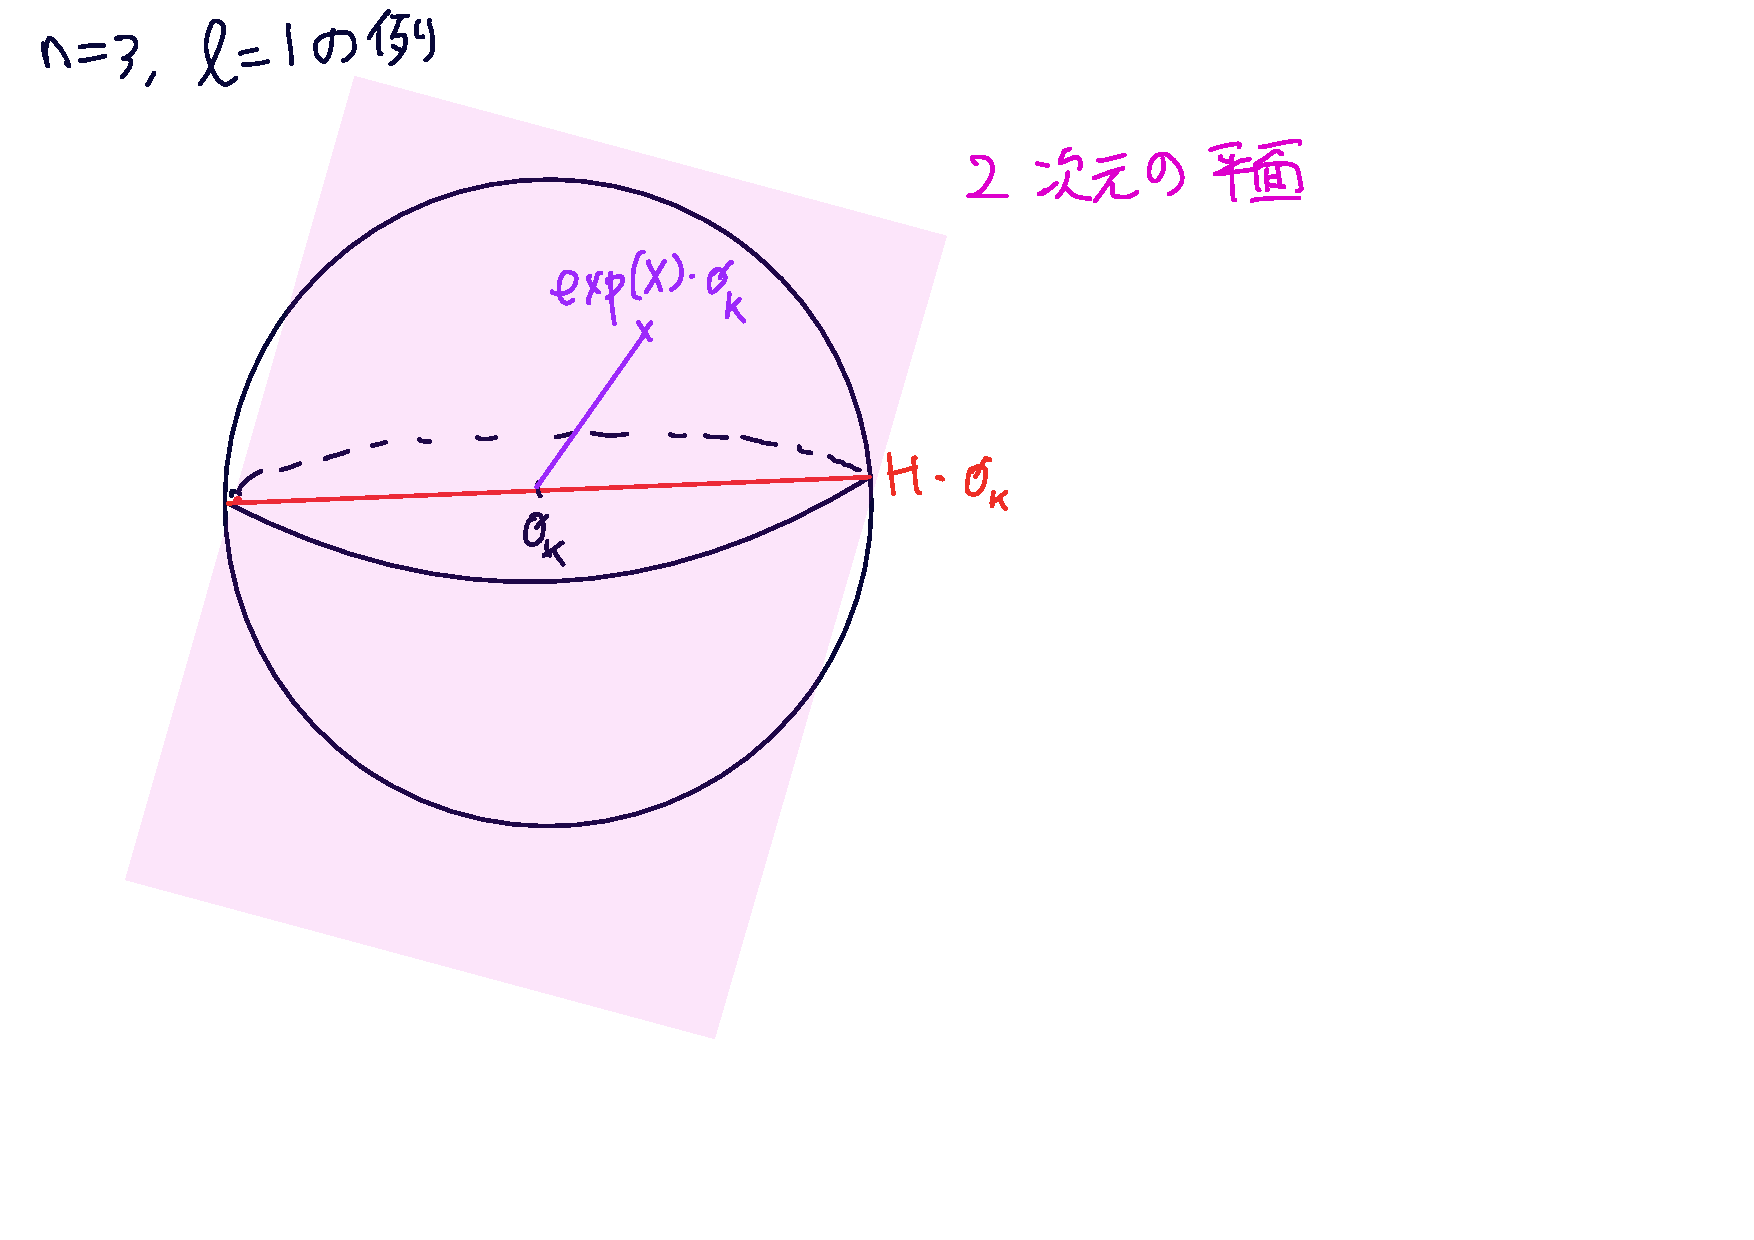
\includegraphics[scale=0.4]{../graph/son1-5.pdf}
  %   \caption{}
  %   \label{fig:son1}
  % \end{figure}
  
  % この断面に現れるのは\Cref{fig:prob-eg-1}と同様の{\Poincare}円板 (Riemann計量は定数倍で変わりうる) であるから,同様の計算により\Cref{cor:prob-eg}を得る.

  % よって\Cref{lem:1018}より,$\norm{Y(X)} = \frac{s}{2} = \frac{1}{4}\inv{\tanh}(\cos\theta \tanh 2t) $を得る.再び\Cref{lem:1018}より$4\norm{X} = 2t $であるから,$\norm{Y(X)} = \frac{1}{4}\inv{\tanh}[\tanh(4\norm{X})\cos\theta] $を得,\Cref{thm:1018-main}の主張が従う.  
\end{npfwn}


%%% Local Variables:
%%% mode: latex
%%% TeX-master: "okuda-master-thesis"
%%% End:
